%%This chapter is used to show our implementation in ProM.  It can be split into 3 parts. 
%The first one is the Dfg method, including the weight update, process tree generation and petri net without long-term dependency generation.
% The second part is to add long-term dependency, it can be use as whole part or customized part into model, also removing the long-term dependency
% Evaluation part is the confusion matrix measurement.
%% Change implementation structure in this way::
%% 1. platform introduction, ProM + KNIME platforms
%% 2. No neccessary to describe the input right?? Aslo, there are another new concepts shown in the graph, which we need to avoid it. 
%% 3. then the screenshots to show the steps of the implementation
%% 4. If we introduce the property here, really, it will not help.. In this way, it can be fine.. But just add the introduction part for the KNIME
In this chapter, we begin with the introduction of implementation platforms for our methods and then show the use of those applications step by step.

\section{Implementation Platforms}
\subsection{Process Mining Platform -- ProM}
ProM is an open-source process mining tool in Java that is extensible by adding a set of plug-ins\cite{ProM}. ProM supports a wide variety of process mining techniques and is usually used for academic research. We implement the algorithm on ProM 6.8, which is the latest stable version. The corresponding plugin is \textbf{\emph{Repair Model By Kefang}} and released online\cite{MyPlugin}.

\subsection{KNIME}
KNIME Analytics Platform is an open-source software to help researcher analyze data by integration of multiple modules for loading, process and transformation and machine learning algorithms. Researcher can achieve their goals by creating visual workflows composed of modules implemented as nodes with an intuitive, drag and drop style graphical interface, rather than focusing on any particular application area.

The reasons to integrate our techniques into KNIME are (1)KNIME is widely used in scientific research and benefits the application of our techniques;(2)KNIME supports automation of test workflow, which helps conduct more efficient experiments.  However, the integration requires additional development effort.
% here we need to change the name of our sections, because if we present them into a general way, so we need to show them in a general methods.
\section{Generate A Process Model}
Firstly the dialog for options to generate directly-follows graphs from event log pops up. Event classifier are set by those dialogs. Subsequently, a dialog is shown to set the Inductive Miner parameters. The parameters include the Inductive Miner variant and the noise threshold to filter the data. The dialog is displayed in Figure \ref{fig:dfg-IM-setting}.
\begin{figure}
	\centering
	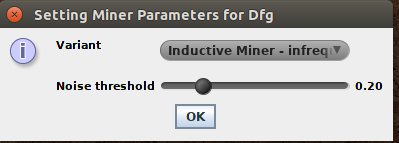
\includegraphics[scale=0.75]{figures/implementation/dfg-IM-setting.png}
	\caption{Inductive Miner Parameter Setting}
	\label{fig:dfg-IM-setting}
\end{figure} \\
After setting the parameters, process models  of process tree and Petri net without long-term dependency can be generated by Inductive Miner and displayed in the result view in Figure \ref{fig:dfg-IM-pn-without-lt}. 
\begin{figure}
	\centering
	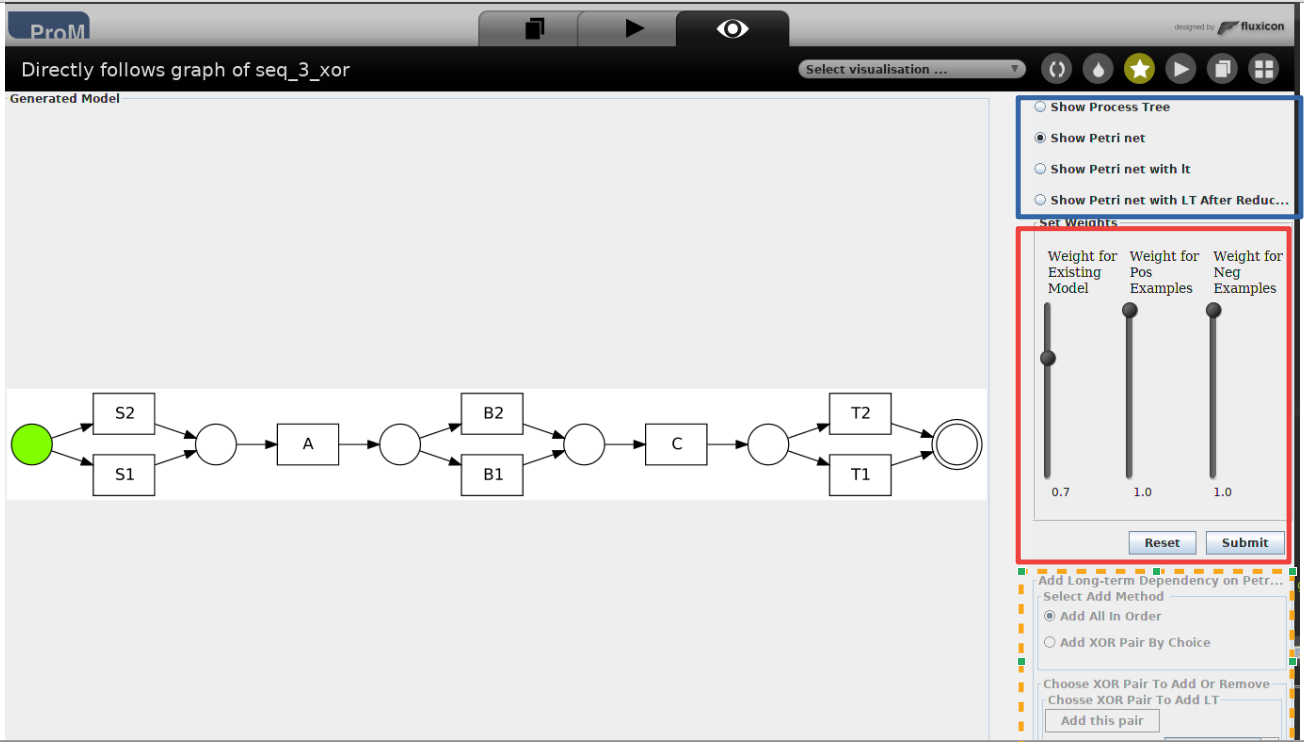
\includegraphics[width=\textwidth]{figures/implementation/dfg-IM-pn-without-lt.png}
	\caption{Generated Petri net without long-term dependency}
	\label{fig:dfg-IM-pn-without-lt}
\end{figure}
The left side is the model display area. To allow more flexibility, this plug-in are interactive by the control panel, which is the right side of result view. Originally, only the generated model type and the weight sliders are enabled, while the control panel for adding long-term dependency are invisible. 

The model type are in the blue rectangle marked in Figure \ref{fig:dfg-IM-pn-without-lt}. It has 4 options to control the generated model type. Currently, the option "Show Petri net" is chosen, so the constructed model is Petri net without long-term dependency. The weights sliders are in red rectangle. It enables to adjust the weights on the existing model, positive and negative instances. Once submitted those options, different process models are mined under different weights. The rectangle in orange are the invisible part to control long-term dependency options. It is discussed in the next section.

\section{Post Process to Add Long-term Dependency }
If the model ro generate is Petri net with long-term dependency, the program to add long-term dependency is triggered. This program in the background detects and puts places and silent transitions on Petri net directly mined from Inductive Miner to add long-term dependency. As comparison, the same weight setting is kept like the Figure \ref{fig:dfg-IM-pn-without-lt}, but the option to show a Petri net with long-term dependency is chosen. The resulted model is Figure \ref{fig:dfg-IM-pn-with-lt}. 
\begin{figure}
	\centering
	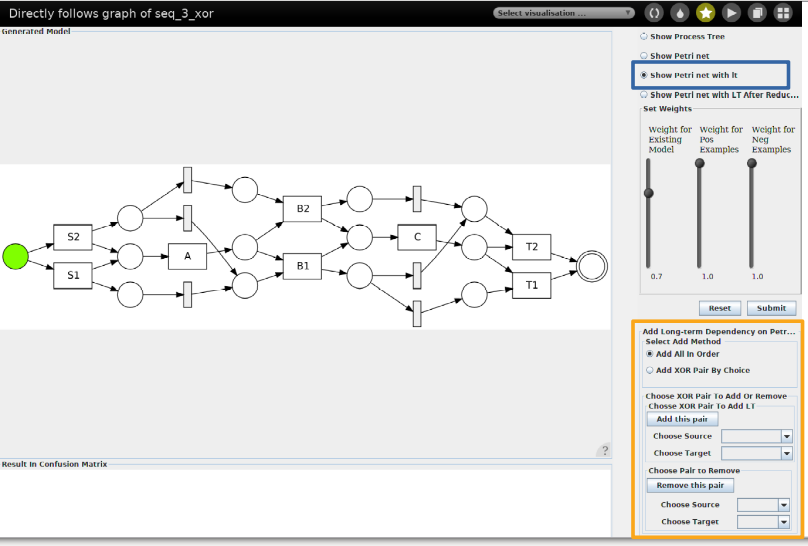
\includegraphics[width=\textwidth]{figures/implementation/dfg-IM-pn-with-lt.png}
	\caption{Petri Net with long-term dependency }
	\label{fig:dfg-IM-pn-with-lt}
\end{figure}

Meanwhile, the control part of adding long-term dependency turns visible, which is in the orange rectangle in Figure \ref{fig:dfg-IM-pn-with-lt}.  It has two main options, one is to consider all long-term dependency existing in the model, the other is to choose the part manually. It allows more flexibility for users. Below those two options, it is the manual selection panels, including control part to add and remove pair. As an example, the blocks Xor(S1,S2) and Xor(T1,T2) are chosen to add long-term dependency. It results in the model in Figure \ref{fig:dfg-IM-pn-with-lt-m}. 
\begin{figure}
	\centering
	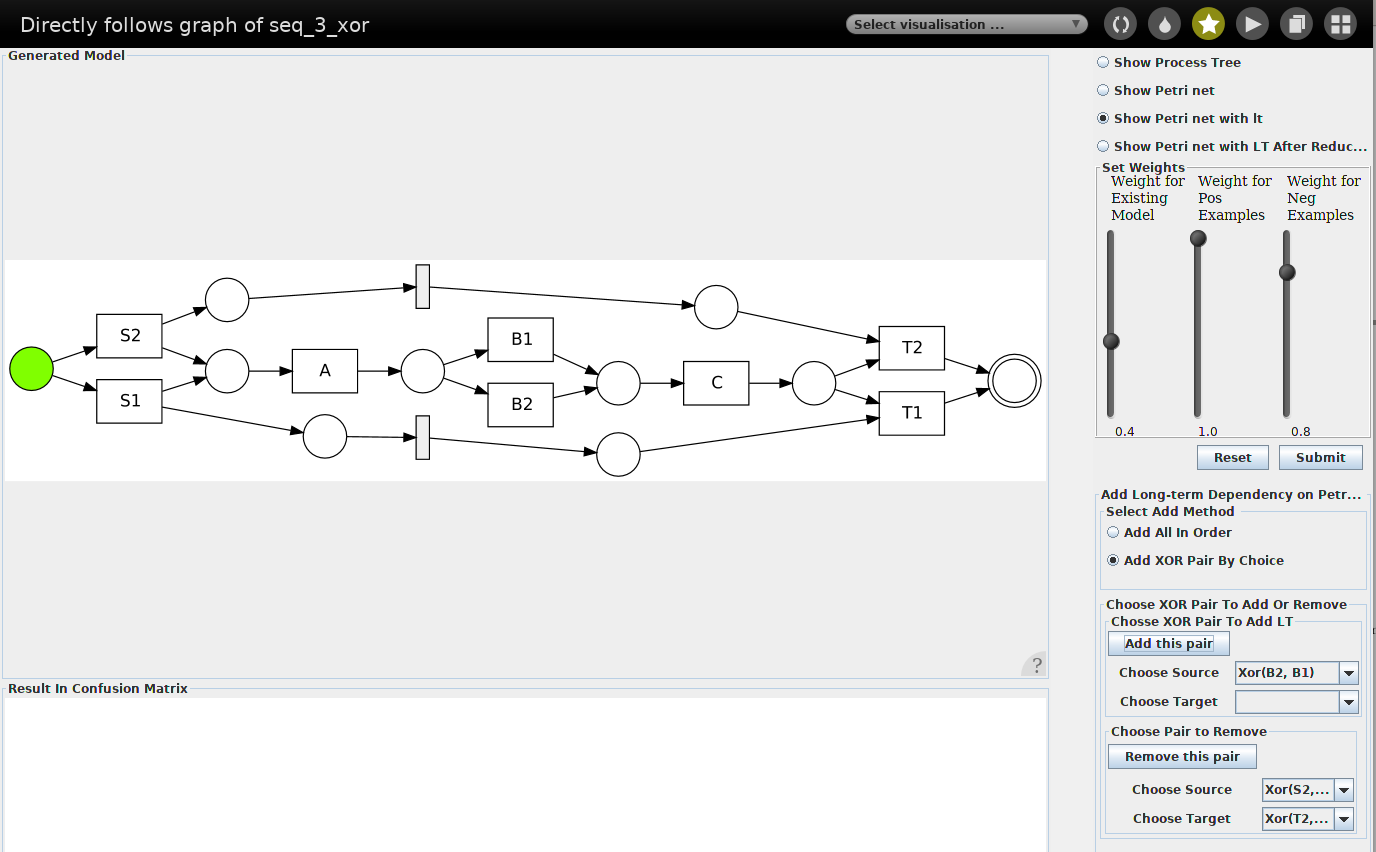
\includegraphics[width=\textwidth]{figures/implementation/dfg-IM-pn-with-lt-manual.png}
	\caption{Petri net with selected long-term dependency}
	\label{fig:dfg-IM-pn-with-lt-m}
\end{figure}
\section{Post Process to Reduce Redundant Silent Transitions and Places}
By choosing \emph{Petri net with LT After Reducing} in model type option panel, silent transitions are reduced to simplify the model.
Under the same setting in Figure \ref{fig:dfg-IM-pn-without-lt}, the simpler model in Figure \ref{fig:dfg-IM-pn-with-lt-r} is constructed, after the post processing of reducing silent transitions.
\begin{figure}
	\centering
	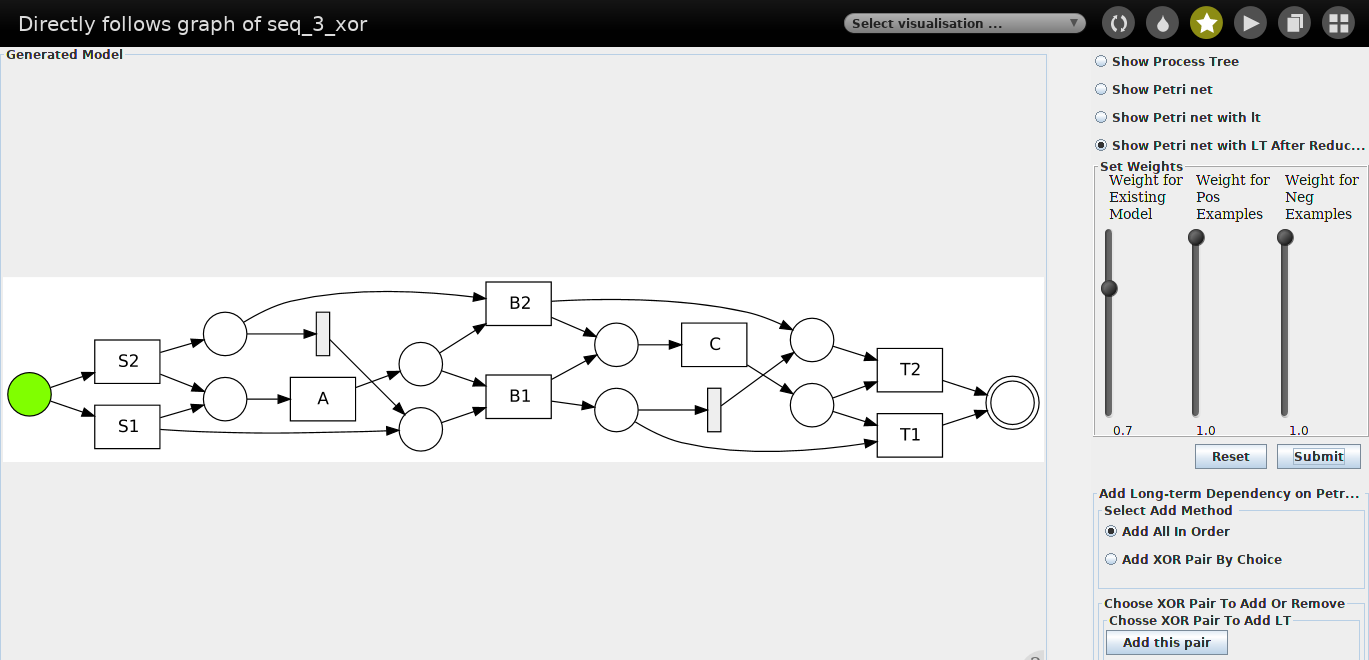
\includegraphics[width=\textwidth]{figures/implementation/dfg-IM-pn-with-lt-reduced.png}
	\caption{Petri net after reducing the silent transitions}
	\label{fig:dfg-IM-pn-with-lt-r}
\end{figure}

\section{Additional Feature to Show Evaluation Result}
Another feature in this plugin  is to show the evaluation result based on confusion matrix. With the brief evaluation result, it helps set the parameter and select the final process model. 

It works in this way. After creating the current model in the left view, the evaluation program in background uses the event log and the current Petri net in the view as inputs. It applies a naive fitness checking and generates a confusion matrix with relative measurements like recall, precision. This evaluation result is then shown in the bottom of the left view in Figure \ref{fig:dfg-IM-cm}.  If the button of green rectangle in the right view \emph{Show Confusion Matrix} is pressed again, the program is triggered again and generates a new  confusion matrix result in  dark green dashed rectangle which will be listed above the previous result in light green dashes area. 
\begin{figure}
	\centering
	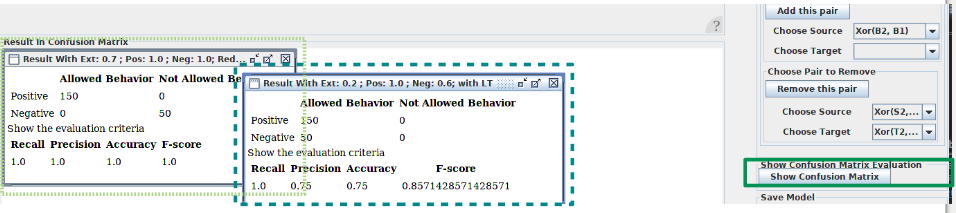
\includegraphics[width=\textwidth]{figures/implementation/dfg-IM-confusionmatrix.png}
	\caption{Generated Process Tree Model}
	\label{fig:dfg-IM-cm}
\end{figure}

\section{Integration into KNIME}
% this section describes the integration of our algorithm with KNIME, should we introduce some parts abotu them?? Yes, here about our real implementation, above should introduce the basic implementation steps.
To integrate our algorithm into KNIME, other related modules on process mining are necessary, which can be divided into the following categories: (1) event log and process models importer and exporter; (2) event logs manipulation;(3)classic discovery algorithms;(4) model enhancement with the algorithm in this thesis. 

\emph{Nodes} in the workflow represents different modules corresponding the plugins in ProM. Each node has certain input ports on the left side to represent the required parameters and  ports on the right to output result. By connecting the ports between nodes, data are passed and processed by one node after another.
 
To integrate our repair algorithm from ProM into KNIME, we need to create the workflow in the Figure \ref{fig:impl-KNIME}. After reading a Petri net by  \emph{PetrinetReader} and an event log by \emph{Import Event Log(XES)}, Node \emph{IncorporateNegInfo} applies the algorithm in this thesis to repair a model in Petri net with incorporating negative information. The outputs have different kinds of Petri nets to match the ones generated in ProM, eg. reduced Petri net with long-term dependency, Petri net without long-term dependency. At last, to obtaining the feature of showing evaluation result, the node \emph{RepairEvaluator} is called. What's more, we can save our Petri net by using node \emph{PetrinetWriter}.
% give a screen shot and list the explaination on it.
\begin{figure}
	\centering
	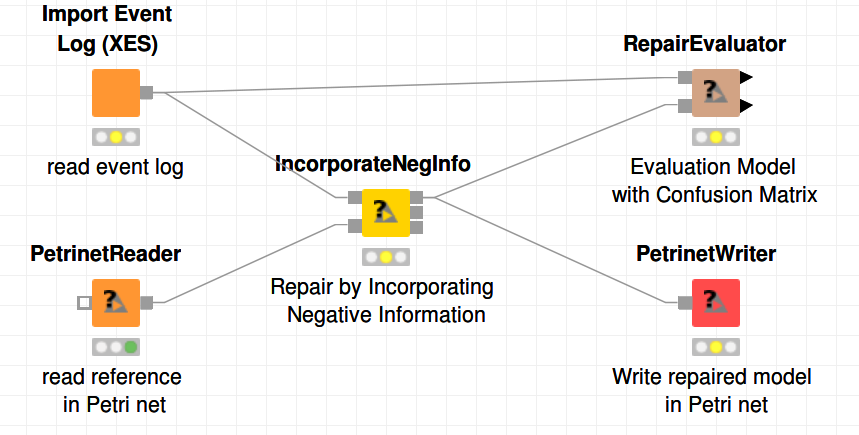
\includegraphics[width=\textwidth]{figures/implementation/implementation-KNIME.png}
	\caption{Integration of our repair techniques into KNIME}
	\label{fig:impl-KNIME}
\end{figure}
